

    Am Anfang jedes neuen Projektes in der Softwareentwicklung muss die Entscheidung getroffen werden, wie qualitativ gut die Software am Ende sein soll.
    Damit sind die Eigenschaften/Funktionalitäten der Software gemeint, die für die Benutzer irrelevant sind, jedoch eine sehr große Bedeutung 
    für das Entwicklungsteam haben.
    
    In der nachfolgenden Tabelle werden die Software, in die unterschiedliche Menge an Zeit inverstiert wurde.

    \begin{tabular}{ |l|c|c| } 
        \hline
                                                                & viel Zeit & wenig Zeit \\ 
                                                                \hline
        Bugs fixen                                              & schnell       & langsam \\ 
        Neue Funktionalität integrieren                         & schnell       & langsam \\
        Änderungen umsetzen                                     & schnell       & langsam \\ 
        Einarbeitungszeit                                       & gering        & groß \\
        Wahrscheinlichkeit alte Funktionalitäten kaputt zu machen & klein       & groß \\
        \hline
       \end{tabular}

    % Eine qualitativ gute Software besitzt unteranderem folgende Vorteile:
    % \begin{itemize}
    %     \item Bugs können schneller lokalisiert und beseitigt werden
    %     \item Neue Funktionalitäten können mit weniger Aufwand umgesetzt werden
    %     \item Die Änderungen der Funktionalitäten können schneller umgesetzt werden
    %     \item Die Wahrscheinlichkeit bestehende Funktionalitäten ungewollt zu ändern veringert sich
    %     \item Die Einarbeitungszeit von neuen Teammitgliedern verkürzt sich 
    % \end{itemize}

    Um diese Vorteile zu erhalten, muss regelmäßig Zeit in folgende Tätigkeiten inverstieren:
    \begin{itemize}
        \item Durchführen von Code Refactoring
        \item Überprüfen der Code Qualität
        \item Durchführen von Code Reviews
        \item Erstellen automatisierte Tests (Unit-, Integration- und Systemtests)
        \item Dokumentation aktualisieren
        \item Technischen Schulden gering halten
    \end{itemize}

    Nicht in jedem Projekt ist das Umsetzen von oben genannten Eigenschaften möglich, 
    da meißt entweder die Zeit oder das Budget oder beides zu gering sind.
    Mit Hilfe folgender Kriterien können einfacher Entscheidung getroffen werden:
    \begin{itemize}
        \item Wann soll die erste Version der Anwendung vorhanden sein.
        \item Wie hoch ist die Anzahl der zur Verfügung stehenden Ressourcen
        \item Wie wahrescheinlich sind die Änderungen und Erweiterungen der Software
        \item Wie kritisch verschiede Probleme und Ausfälle der Software sind 
    \end{itemize}

    In der Abbildung \ref{fig:softQuality} ist zu erkennen, dass auf längerer Distanz eine gute Softwarearchitektur deutlich mehr Funktionalitäten 
    besitzt als eine Software mit schlechter Architectur. Im vorderen Zeitinterval führt allerdings die Software mit der qualitativ schlechteren Architektur.
    \begin{figure}[H]
        \centering
        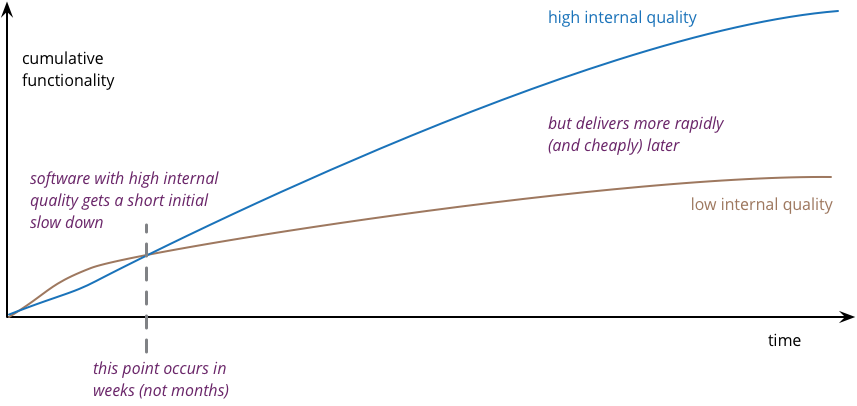
\includegraphics[width=1\textwidth]{./images/QASoftwareCompare.png}
        \caption[Vergleich einer guten und einer schlechten Softwarearchitektur]{Vergleich einer guten und einer schlechten Softwarearchitektur \footnotemark}
        \label{fig:softQuality}
    \end{figure}
    \footnotetext{https://martinfowler.com/bliki/DesignStaminaHypothesis.html}
    Diesen Verlauf ist beim Projektbegin zu beachten. Es ist nicht vom Vorteil bei einem Projekt, 
    für das man nur eine Woche Zeit hat, eine gute Architektur zu implementieren, die ohne jeglichen Funktionalitäten mehrere Wochen gebrauchen wird.

    Wenn das Projekt regelmäßig weiterentwickeln wird, ist es vom Vorteil gleich eine gute Architektur umzusetzen.
